% This is the magic command for latextools(ST3)
%! TEX program = latexmk -xelatex
\XeTeXgenerateactualtext=1

%%%%%%%%%%%%%% 文字コードについて %%%%%%%%%%%%%%
% Windows では標準で文字コードが Shift-JIS に  %
% である事が多いが,TeX のソースコードは UTF-8 %
% 書くことを推奨する                           %
%%%%%%%%%%%%%%%%%%%%%%%%%%%%%%%%%%%%%%%%%%%%%%%%

% 行頭に '%' をつけるとコメントになる

%%% ドキュメントクラスの設定 %%%
% 基本的にここは変更しない
% 文章全体の文字サイズを変えたい場合は 'XXpt' を変更すること
% デフォルトの文字サイズは10pt
\documentclass[a4paper, twocolumn, xelatex, 10pt, ja=standard, Ligatures=TeX]{bxjsarticle}

%%% プレアンブル ---ここから %%%

% Preamble.tex のインポート
% This is the magic command for latextools(ST3)
%!TEX root = ./Report.tex

%%%%%%%%%%%%%%%%%%%%%%%%%%%%%%%%%%%%%%%%%%%%%%
%%%%%%%%%%%%%%%  各種設定  %%%%%%%%%%%%%%%%%%%
%%%%%%%%%%%%%%%%%%%%%%%%%%%%%%%%%%%%%%%%%%%%%%

\setpagelayout{top=20truemm, bottom=20truemm, left=12truemm, right=12truemm}

\usepackage{xeCJK}
\usepackage{graphicx}
\usepackage{xcolor, color}
\usepackage{here}
\usepackage{ascmac}
\usepackage[hyphens]{url}
\urlstyle{tt}

%%%%%%%%%%%%%%%%%%%%%%%%%%%
%%% フォント指定(XeTeX) %%%
%%%%%%%%%%%%%%%%%%%%%%%%%%%

%% 1. macOS ユーザー向け設定
%% Hiragino, Helvetica, TimesNewRoman, RictyDiminishedDiscord  
	% \usepackage{fontspec}
	% % serifフォント(日本語)
	% \setCJKmainfont[BoldFont={HiraginoSans-W6}]{HiraMinProN-W3}
	% % sans-serifフォント(日本語)
	% \setCJKsansfont[BoldFont={HiraginoSans-W6}]{HiraginoSans-W3}
	% % serifフォント(欧文)
	% \setmainfont[ItalicFont={HelveticaNeue-LightItalic}, BoldFont={HelveticaNeue-Medium}, BoldItalicFont={HelveticaNeue-MediumItalic}]{TimesNewRomanPSMT}
	% % sans-serifフォント(欧文)
	% \setsansfont[ItalicFont={HelveticaNeue-LightItalic}, BoldFont={HelveticaNeue-Medium}, BoldItalicFont={HelveticaNeue-MediumItalic}]{HelveticaNeue-Light}

	% \setmonofont[ItalicFont={RictyDiminishedDiscord-Oblique}, BoldFont={RictyDiminishedDiscord-Bold}, BoldItalicFont={RictyDiminishedDiscord-BoldOblique}]{RictyDiminishedDiscord-Regular}
	% \setCJKmonofont[ItalicFont={RictyDiminishedDiscord-Oblique}, BoldFont={RictyDiminishedDiscord-Bold}, BoldItalicFont={RictyDiminishedDiscord-BoldOblique}]{RictyDiminishedDiscord-Regular}

% 2. NotoSansCJKjp、NotoSerifCJKjp、NotoSans、NotoSerif、RictyDiminishedDiscord
	\usepackage{fontspec}
	% serifフォント(日本語)
	\setCJKmainfont[BoldFont={NotoSansCJKjp-Medium}]{NotoSerifCJKjp-Light}
	% sans-serifフォント(日本語)
	\setCJKsansfont[BoldFont={NotoSansCJKjp-Medium}]{NotoSansCJKjp-Light}
	% serifフォント(欧文)
	\setmainfont[ItalicFont={NotoSerif-LightItalic}, BoldFont={NotoSerif-Medium}, BoldItalicFont={NotoSerif-MediumItalic}]{NotoSerif-Light}
	% sans-serifフォント(欧文)
	\setsansfont[ItalicFont={NotoSans-LightItalic}, BoldFont={NotoSans-Medium}, BoldItalicFont={NotoSans-MediumItalic}]{NotoSans-Light}

	\setmonofont[ItalicFont={RictyDiminishedDiscord-Oblique}, BoldFont={RictyDiminishedDiscord-Bold}, BoldItalicFont={RictyDiminishedDiscord-BoldOblique}]{RictyDiminishedDiscord-Regular}
	\setCJKmonofont[ItalicFont={RictyDiminishedDiscord-Oblique}, BoldFont={RictyDiminishedDiscord-Bold}, BoldItalicFont={RictyDiminishedDiscord-BoldOblique}]{RictyDiminishedDiscord-Regular}


% 日付フォーマット変更
\renewcommand{\today}{\the\year/\the\month/\the\day}

% \maketitle カスタマイズ
\usepackage{titling}
\pretitle{
	\vspace{-2.3cm} % タイトルを上に詰める
	\begin{center}
		\huge\sffamily % タイトル:hugeサイズ、ゴシック体
}
\posttitle{
	\end{center}
}
\preauthor{
	\vspace{\baselineskip}
	\begin{center}
		\large\sffamily % 著者名:largeサイズ、ゴシック体
}
\postauthor{
	\end{center}
}
\predate{
	\begin{center}
		\large\sffamily % 日付:largeサイズ、ゴシック体
}
\postdate{
	\end{center}
}


% セクションのスタイル変更
\usepackage{titlesec}
\titleformat*{\section}{\Large\bfseries\sffamily}
\titleformat*{\subsection}{\normalsize\bfseries\sffamily}


% 参照マクロ
\newcommand{\fref}[1]{\textbf{図\ref{#1}}}
\newcommand{\Fref}[1]{\textbf{式\ref{#1}}}
\newcommand{\tref}[1]{\textbf{表\ref{#1}}}


% listings 設定
% listings: ソースコードを表示するためのプラグイン
\usepackage{listings}

% コード部分の色スタイルの設定
\definecolor{bkg}{gray}{0.95}
\definecolor{def}{gray}{0.00}
\definecolor{com}{gray}{0.60}
\definecolor{key}{rgb}{0.00, 0.00, 0.75}
\definecolor{str}{rgb}{0.20, 0.50, 0.15}

% ソースコードを表示するときのキャプション名
\renewcommand{\lstlistingname}{コード}

% 書式設定
\lstset{
   % プログラミング言語
   language={C},
   % 背景色
   backgroundcolor={\color{bkg}},
   % 基本の文字スタイル
   basicstyle={\small\ttfamily\color{def}},
   % 変数の文字スタイル
   identifierstyle={\small\ttfamily\color{def}},
   % コメントの文字スタイル
   commentstyle={\color{com}},
   % 予約語の文字スタイル
   keywordstyle={\bfseries\color{key}},
   % 非予約語の文字スタイル (よくわからない)
   ndkeywordstyle={\small\color{def}},
   % 文字列リテラルのスタイル
   stringstyle={\bfseries\color{str}},
   % 枠線の設定
   % t, r, b, l: それぞれ上、右、下、左の1本線
   % T, R, B, L: それぞれ上、右、下、左の2本線
   frame={tlRB},
   % 長い文を改行するかどうか
   breaklines=true,
   % 横幅間隔の調整
   columns=[l]{fullflexible},
   % 左右のマージン
	 xrightmargin=0\zw,
   xleftmargin=1\zw,
   framexleftmargin=3pt,
   % 行番号の位置
   numbers=left,
   % 行番号のスタイル
   numberstyle={\ttfamily\small},
   % 行番号とコード本文の間の空白
	 numbersep=1\zw,
   % 行番号の刻み
   stepnumber=1,
   % コメント行の継続の設定
	morecomment=[l]{//}
}
\newcommand{\cref}[1]{\textbf{\lstlistingname\ref{#1}}}


% 行間隔の変更 (0.90倍に)
% \renewcommand{\baselinestretch}{0.90}

%%% プレアンブル ---ここまで %%%

%%% タイトル,筆者,日付の設定 %%%
% \title{\vspace{-1cm}\LARGE ドローン空撮映像を用いた被災状況地図作成支援}
% \author{\vspace{-1cm}静岡大学院\ 総合科学技術研究科\ 情報学専攻\ 佐治研究室 \\ 7113-0054\ 室永\ 将門}
% \date{}
\title{\LARGE ドローン空撮映像を用いた被災状況地図作成支援}
\author{静岡大学院\ 総合科学技術研究科\ 情報学専攻\ 佐治研究室 \\ 7113-0054\ 室永\ 将門}
\date{}
% 文字としての空白を入れるときは,
% '\ ' (バックスラッシュ + 半角スペース)
% を入力する


%%%%%%%%%%%%%%%%%%%%%%%%%%%%%%%%%%%%%%%%%%%%%%
%%%%%%%%%%%%%%%%  本文 部分  %%%%%%%%%%%%%%%%%
%%%%%%%%%%%%%%%%%%%%%%%%%%%%%%%%%%%%%%%%%%%%%%

% インデントは必須ではないが,可読性のために
% インデントを推奨する

\begin{document}	
\maketitle

\section{はじめに}
	近年,豪雨による斜面崩壊・浸水被害が多発し,これらの被災箇所を早急に把握することは救助・復旧・二次災害の防止等に有効である.この被害把握に関し,安全な位置からの解析が可能なリモートセンシング技術が注目されている.\\
	\quad リモートセンシング技術による被災領域検出には主に人工衛星,有人航空機(以下,ヘリコプター),無人航空機(以降,ドローン)が用いられる.人工衛星は広範囲の把握が可能であり,画像処理において扱いが容易な直下視点の画像が得られるが,解像度が低く,天候や撮影周期によっては画像が得られないことがある.ヘリコプターは人工衛星に比べ早期に画像を取得でき,解像度が高いが,金銭的コストが非常に高く,周囲に発着場が必要である.また,保有台数が少なく被災箇所を網羅できない可能性があり,悪天候時には出動できないことがある.これに対しドローンは安価かつ迅速に解像度の高い画像の取得が可能であるため,被害箇所の早急な把握に有効である.これらの解析・判読結果を元に,災害現場の被災箇所を地図上にマッピングした,被災状況地図が作成される.被災状況地図は救助・復旧活動の方針決めや被害の全体把握,二次災害の防止等に用いられるため,災害発生後速やかに作成する必要がある.しかし,災害現場では航空機の操縦から解析,被災状況地図作成までの作業が手動によって行われており,労力と時間がかかることが問題となっている\cite{art00}.\\
	\quad 以上を踏まえ,ドローン空撮映像を用いて被災状況地図の作成を支援するシステムの構築を考える.本研究では被災領域のマッピングを半自動的に行うことで,被災状況地図作成の簡易化を目的とする.

\section{提案手法}
	提案手法の概要図を\fref{img01}に示す.提案手法ではドローン空撮映像からオルソ画像を作成し,被災領域の検出を行う.最後に,地図データと重ね合わせることで被災領域地図を作成する.
	
\begin{figure}[b]
	\centering
		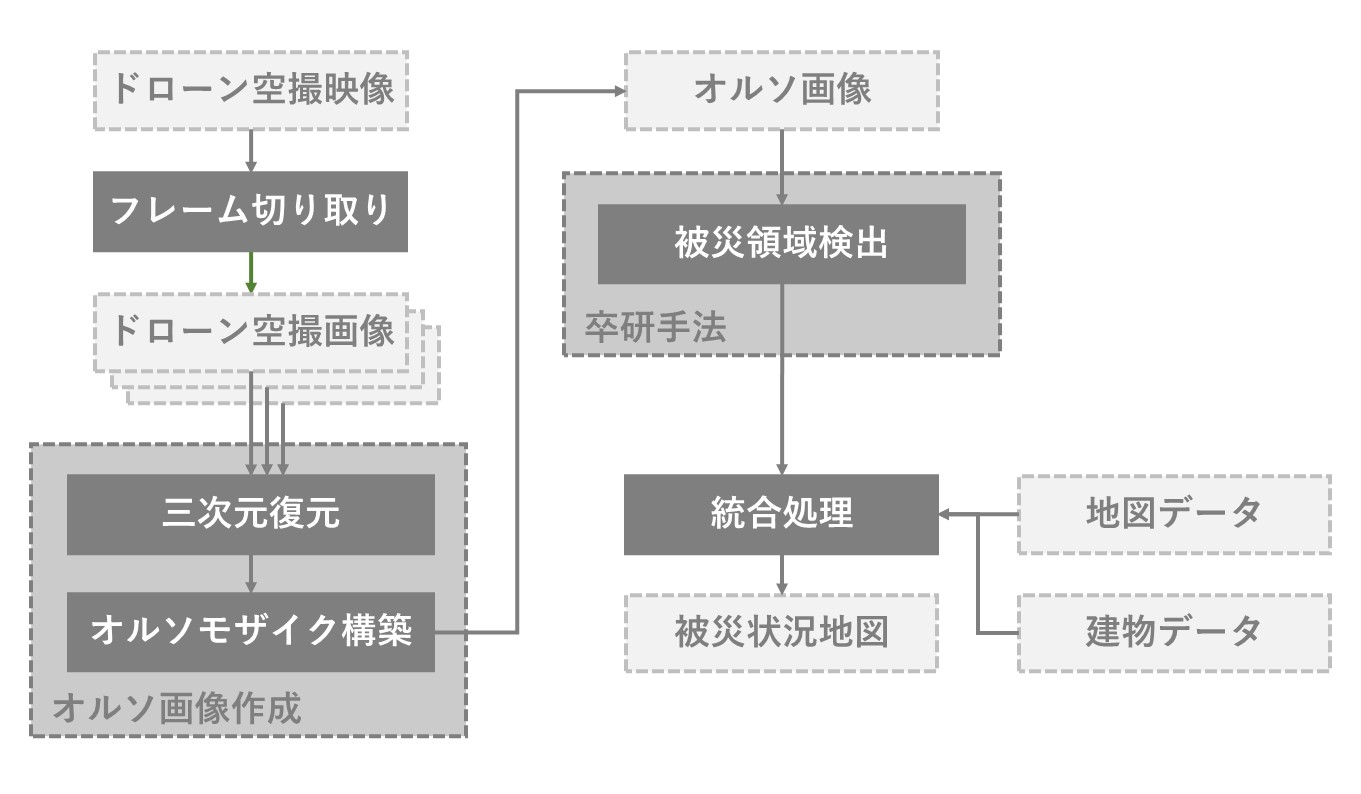
\includegraphics[width=8cm]{img/howto.jpg}
		\caption{提案手法概要図}
		\label{img01}
\end{figure}

\subsection{三次元復元}
	空撮映像からオルソ画像を作成するためには,SfM(Structure from Motion)技術を用いて三次元復元を行い,三次元モデルを生成する必要がある.Agisoft社のMetashapeに映像のフレーム画像を多数入力することで三次元モデルを生成する.

\subsection{オルソモザイク構築}
	SfM技術によって生成した三次元モデルにオルソモザイク構築を行うことで,オルソ画像が得られる.空撮映像のような斜め視点画像の場合,建物等によって地表面の様子が確認できないことがある.これに対し,オルソ画像は直下視点画像であるため,このようなオクルージョンが解消される.
	
\subsection{被災領域検出}
	各被災領域の特徴を\tref{tab01}に示す.これらの特徴を用いて各領域の検出を行う.

	\begin{table}[b]
		\centering
		\caption{各被災領域の特徴}
		\label{tab01}
		\begin{tabular}{c c c c c}
			\hline
			領域名 & 色相 & 彩度 & 輝度 & 均一度 \\
			\hline
			\hline
			斜面崩壊 & 赤 & 高 & 低 & -- \\
			浸水 & 赤 & 低 & 高 & 高 \\ \hline
		\end{tabular}
	\end{table}

	\subsubsection{斜面崩壊領域}
		斜面崩壊領域は\tref{tab01}に示すように,色相と彩度,輝度に特徴を持つ.よって,これらの特徴を表す指標であるL*a*b*表色系のL*値,a*値とHSV表色系のS値を用いる.L*a*b*表色系は人間の視覚に近い色空間であり色相による分類に有効である.L*値は輝度を表し,赤い画素ではa*値が高く,青い画素ではb*値が,緑の画素ではa*値が低い.HSV表色系は色相,彩度,明度の情報を持つ色空間である.本研究では彩度を表すS値を用いる.ヒストグラム均一化処理後の画像に対しL*a*b*表色系変換とHSV表色系変換を行い,これらの指標を用いた閾値処理により斜面崩壊領域を検出する.
	
	\subsubsection{浸水領域}
		浸水領域は\tref{tab01}に示すように,色相と彩度,輝度,均一度に特徴を持つ.よって,前項同様にL*値,a*値,S値を利用することに加えて,均一度の指標としてエッジの有無を用いることで,領域が滑らかなテクスチャかの判定を行う.このとき,エッジの検出にはCanny法を利用し,領域単位でエッジ抽出率を算出する.そして,色相等の指標と領域単位でのエッジ抽出率による閾値処理によって浸水領域を検出する.

\subsection{統合処理}
	前節にて被災箇所をマッピングしたオルソ画像をデジタル地図上に重ね合わせる.この処理による地図が被災状況地図である.	


\section{実験}
\subsection{実験結果}
	現時点では未実施であるため,理想的な出力結果を示す.ここでの動画像は平成29年7月九州北部豪雨のドローン空撮映像\cite{web01}を用いて国土地理院が作成したものである.\tref{tab03}に空撮映像の詳細を示す.また,\fref{img02}--\fref{img07}に入力画像と各処理の理想的な出力画像を示す.
	
	\begin{table}[b]
		\centering
		\caption{実験データ}
		\label{tab03}
		\begin{tabular}{l l}
			\hline
			災害名称 & 平成29年7月九州北部豪雨 \\
			撮影箇所 & 福岡県朝倉市赤谷川 \\
			撮影日時 & 平成29年7月7日15時30分 \\
			解像度 & 1920 × 1080 pixel \\
			提供 & 国土地理院 \\ \hline
		\end{tabular}
	\end{table}
	
	\begin{figure}[b]
		\begin{minipage}{0.48\hsize}
			\centering
			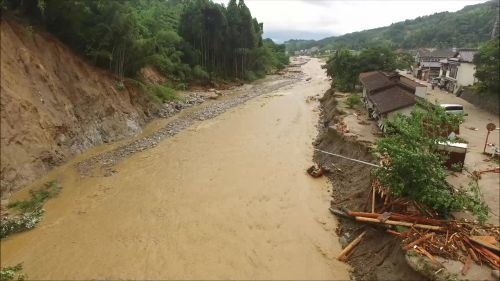
\includegraphics[width=\linewidth]{img/original.jpg}
			\caption{入力映像}
			\label{img02}
		\end{minipage}
		\begin{minipage}{0.48\hsize}
			\centering
			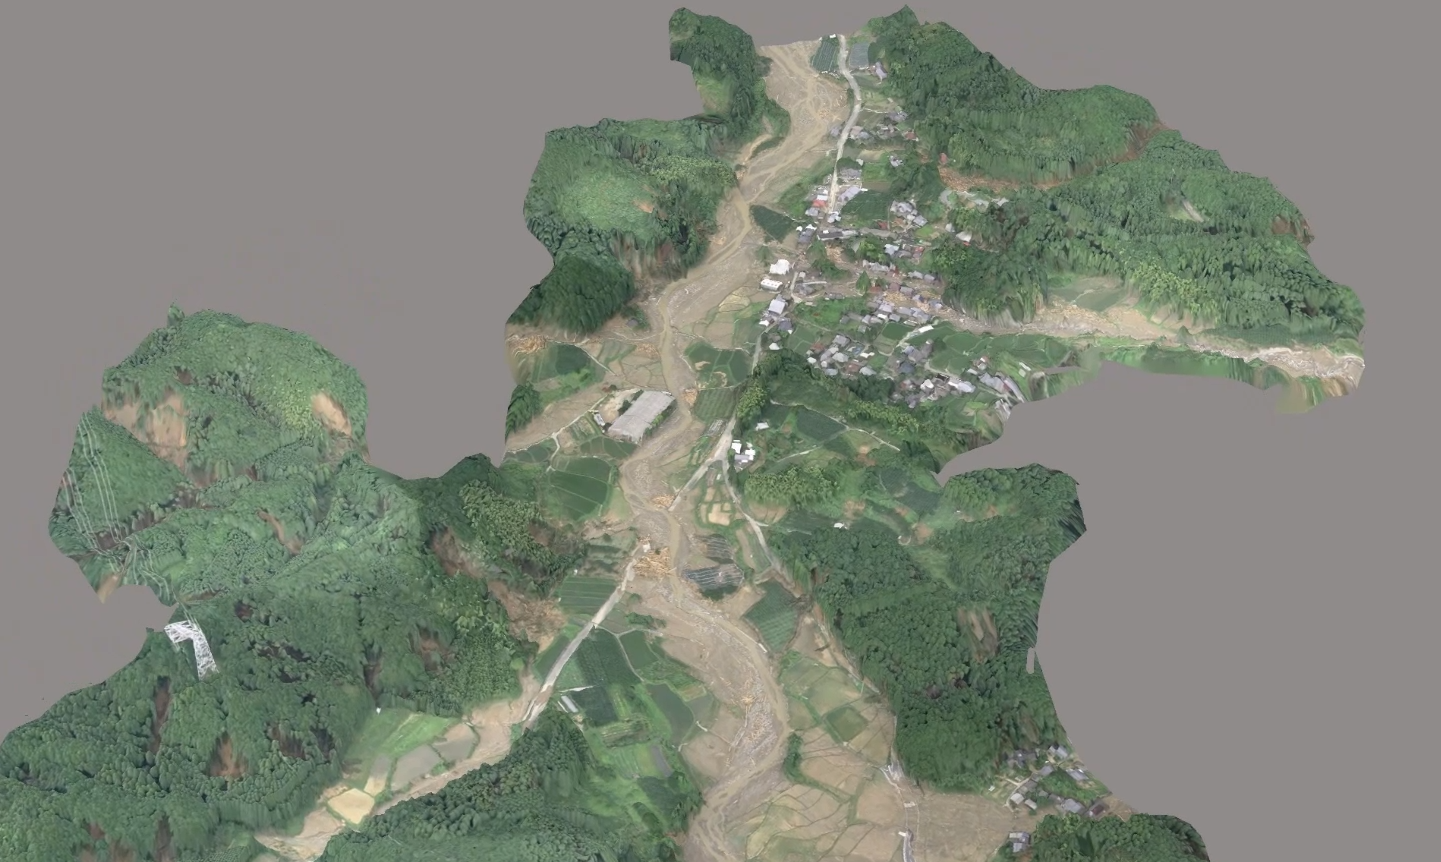
\includegraphics[width=\linewidth]{img/3dmodel.png}
			\caption{三次元復元}
			\label{img03}
		\end{minipage}
	\end{figure}
	\begin{figure}[t]
		\begin{minipage}{0.48\hsize}
			\centering
			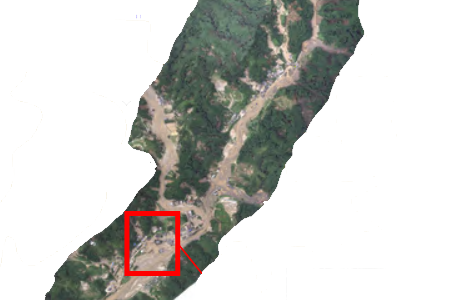
\includegraphics[width=\linewidth]{img/ortho.png}
			\caption{オルソモザイク構築}
			\label{img04}
		\end{minipage}
		\begin{minipage}{0.48\hsize}
			\centering
			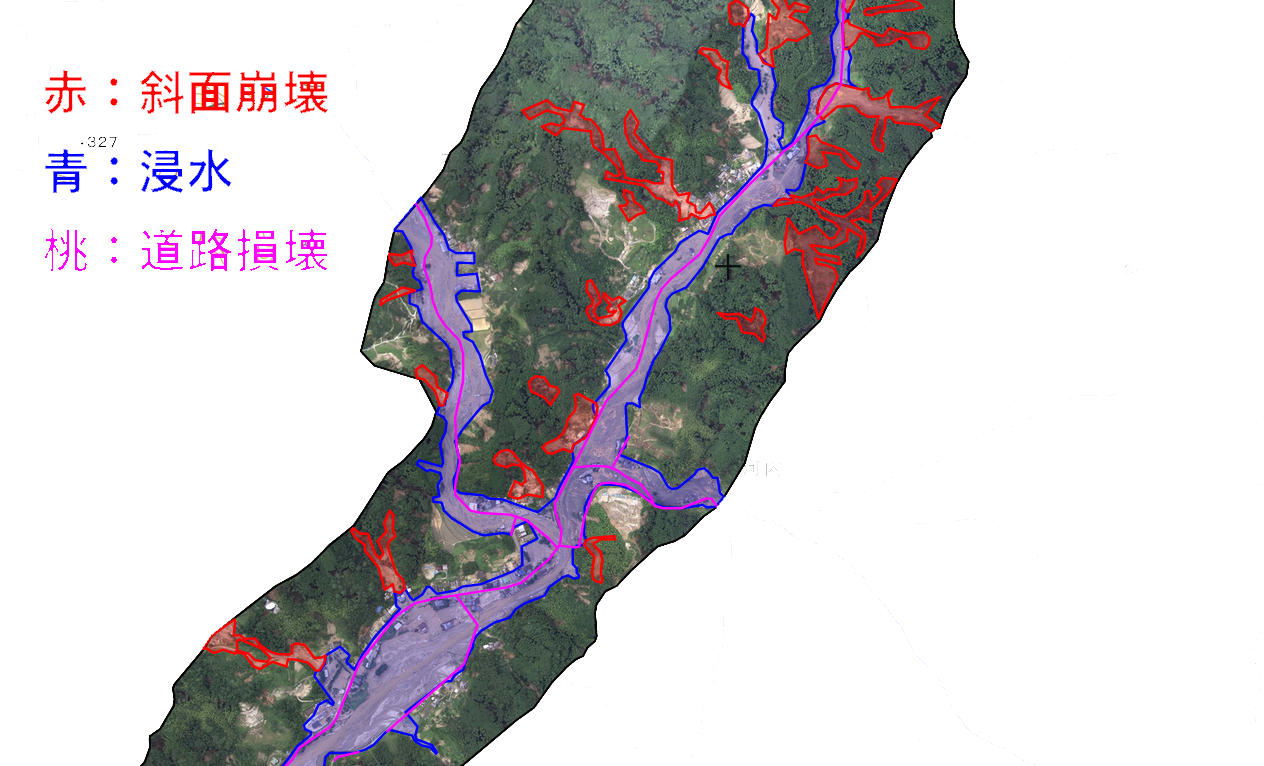
\includegraphics[width=\linewidth]{img/detection.png}
			\caption{被災領域検出(赤:斜面崩壊,青:浸水,桃:道路損壊)}
			\label{img05}
		\end{minipage}
	\end{figure}
	\begin{figure}[t]
		\begin{minipage}{0.48\hsize}
			\centering
			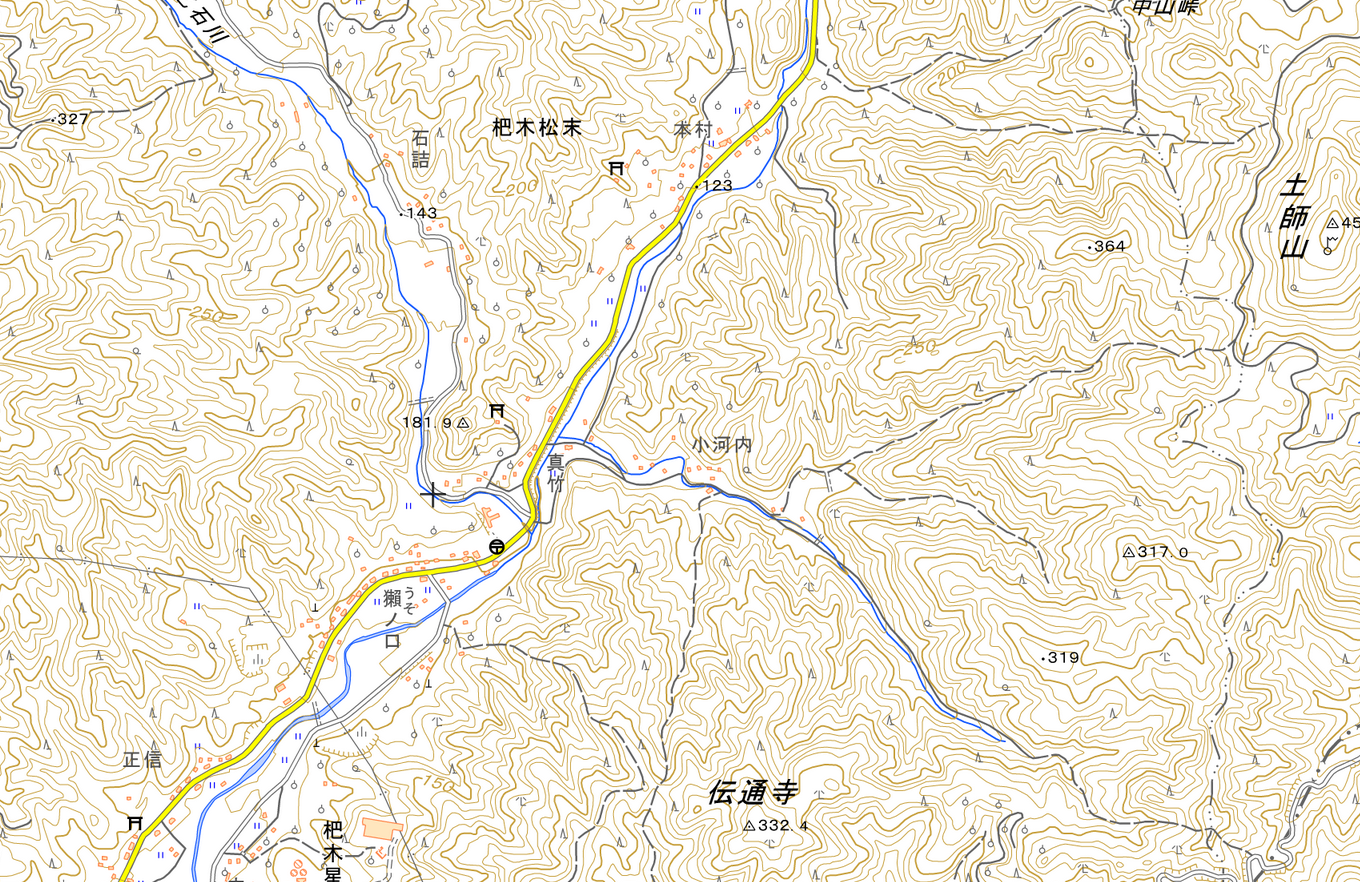
\includegraphics[width=\linewidth]{img/map.png}
			\caption{地図データ}
			\label{img06}
		\end{minipage}
		\begin{minipage}{0.48\hsize}
			\centering
			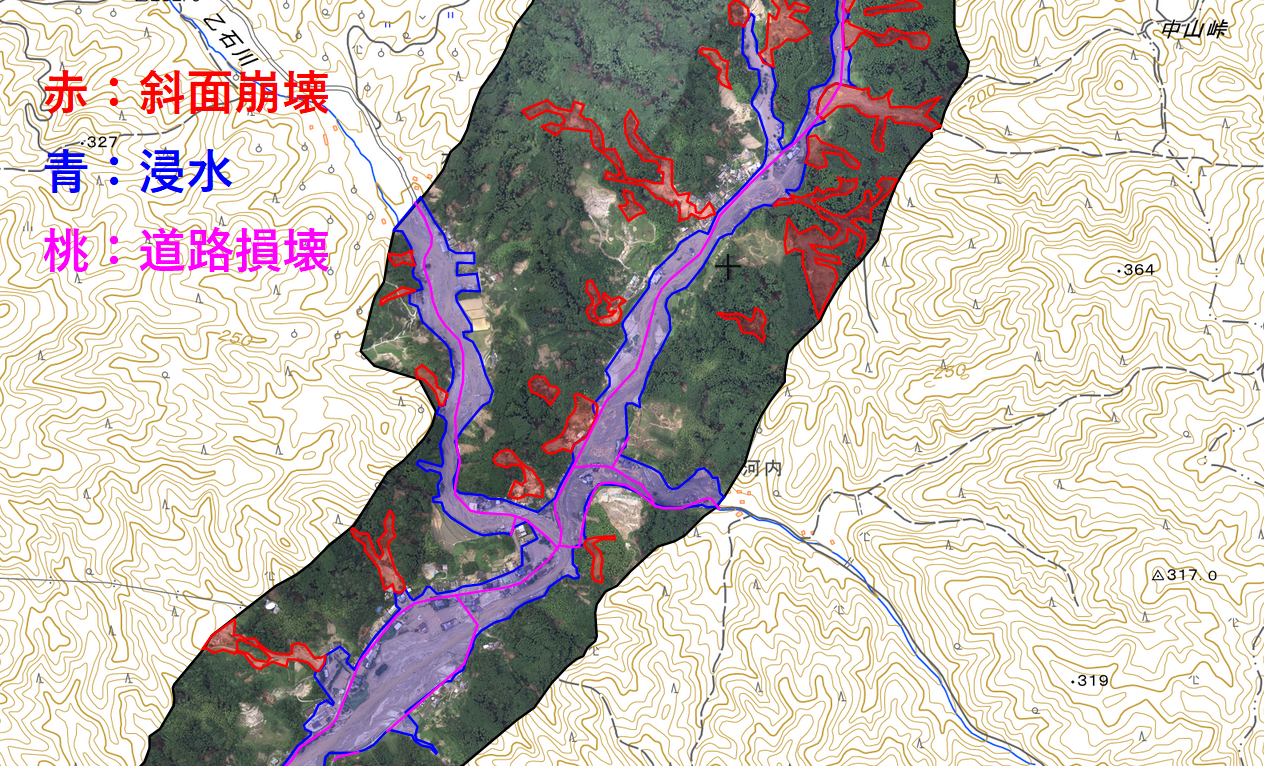
\includegraphics[width=\linewidth]{img/result.png}
			\caption{出力画像(被災領域地図)}
			\label{img07}
		\end{minipage}
	\end{figure}


\section{まとめ・今後の予定}
	本論ではドローン空撮映像から被災領域地図の作成支援手法を提案した.現状では実験を行っていないため,各処理にて理想的な出力となるかは不明である.被災状況地図については,各工程でどの程度自動化の余地があるのか,何をマッピングすれば実際の災害現場で役に立つのかを調査する必要がある.今後はこれらの実装・調査を行う予定である.


\section{参考文献}		
	% 参考文献はbibtexを用いて作成する.文献を参照するには\cite{鈴木:論文06},\cite{Web01}とする.

% 参考文献の表示
\bibliographystyle{junsrt}   % 参考文献の並び順を指定
\bibliography{bib/myref.bib} % \bibliography{参考文献ファイルへのパス}

\end{document}
